\title{\textbf{Haiku}\\OS Report Part I}
\author{COMP 3000\\ \\Troy Hildebrandt -- 100622385\\Nima Hoda -- 100308135}
\date{\today}



\documentclass{article}

\usepackage{cite}
\usepackage{url}
\usepackage{graphicx}
\usepackage{subfig}

% Page setup
% Shamelessly stolen from Pat Morin's Open Data Structures
\setlength{\textheight}{8.5in}
\setlength{\textwidth}{6in}
\setlength{\topmargin}{-0.375in}
\setlength{\oddsidemargin}{.25in}
\setlength{\evensidemargin}{.25in}
\setlength{\headheight}{0.200in}
\setlength{\headsep}{0.4in}
\setlength{\footskip}{0.500in}
\setlength{\parskip}{1.5ex}
\setlength{\parindent}{1.25cm}
%\flushbottom

\newcommand{\figref}[1]{Figure~\ref{fig:#1}}

\begin{document}
\maketitle

\section{Background}

Haiku is a portable \cite{HaikuFaq} free and open source
\cite{HaikuDevFaq} operating system for the 32-bit x86 architecture
\cite{HaikuFaq} targeting personal computing \cite{HaikuAbout}.  It
was originally named OpenBeOS after BeOS \cite{HaikuWiki}, the
short-lived proprietary operating system developed by Be,
Inc. throughout the 1990s, which focused on digital media work
\cite{BeosWiki}.

BeOS boasted an object-oriented C++ API, a fully integrated graphical
user environment, a modern multiprocessing, preemptively multitasking
kernel, a journaling file system with a relational database-like
metadata facility \cite{BFSWiki} and included partial POSIX
compatibility.  However, despite having a devoted niche user base, it
could not yield a profit for Be, Inc. and, in 2001, was acquired by
Palm, Inc., ending further BeOS development \cite{BeosWiki}.

Disapointed with the loss, a group of BeOS enthusiasts began an
effort to rewrite BeOS as a free and open source project
\cite{BeosWiki, HaikuHistoryWiki}.  In 2004 the open source effort was
renamed Haiku, after the three line Japanese form of poetry which
appeared on occasion in BeOS error messages \cite{HaikuFaq,
  HaikuHistoryWiki}.

Haiku takes its inspiration from BeOS \cite{HaikuAbout} and aims to
recreate both the BeOS technologies and end user experience
\cite{HaikuFaq}.  Haiku uses the same window decoration style and
colour as BeOS \cite{HaikuWiki, BeosWiki} and aims to create a
unified, cohesive user interface \cite{HaikuAbout, HaikuHIG,
  HaikuIcon} reflecting the ``core qualities'' of ``elegance'' and
``simplicity'' found in BeOS \cite{HaikuFaq}.  Haiku also directly
incorporates two core BeOS user interface elements, the Tracker, a
file manager, and the Deskbar, a taskbar, which were open sourced by
Be, Inc. in 2001 \cite{HaikuFaq}.  Haiku also reimplements the
object-oriented C++ BeOS API\cite{HaikuWiki} as well as the Be File
System with, its advanced meta-data capabilities \cite{BFSWiki}.

Haiku is targetted towards the personal computer user
\cite{HaikuAbout}.  As such, it includes a fully integrated GUI
environment, rejecting the stacked nature of the X Window System on
UNIX-like operating systems \cite{HaikuFaq}.  The personal computing
focus is also reflected in Haiku's current lack of support for
multi-user operation, though are plans for such support in future
releases \cite{HaikuFuture}.  Haiku also aims to present a unified
human interface, both in terms of the operating system base as well as
in applications developed for Haiku.  This is reflected in the
development and maintenance of comprehensive Haiku human interface and
icon guidelines \cite{HaikuHIG, HaikuIcon}.

Haiku currently only supports the 32-bit x86 architecture, though
ports to other platforms, including x86-64, are being developed and
may be supported in the future \cite{HaikuFaq}.  On 32-bit x86, Haiku
aims for full source and binary compatibility with 32-bit x86 BeOS
applications.  Several major BeOS R5 applications already run
successfully on Haiku, including Opera, Firefox and Quake III
\cite{HaikuWiki}.  POSIX compatibility is also a Haiku goal
\cite{HaikuFuture, HaikuIncContracts}, as are the development of a
BSD-style ports collection \cite{HaikuPorts}, which would simplify the
building of 3rd party open-source software and a full package
management system to manage installation and dependency resolution of
3rd party software \cite{HaikuR1A3Notes}.

Haiku development is centred around the Haiku Project, an
international community of volunteers \cite{HaikuAbout}.  The project
maintains mailing lists, forums, IRC channels, \cite{HaikuComm} source
code repositories \cite{HaikuGetSvn} and several websites, including
the following:
\begin{itemize}
  \item \url{http://www.haiku-os.org/} -- the main project website
  \item \url{http://api.haiku-os.org/} -- containing Haiku API documentation
  \item \url{http://dev.haiku-os.org/} -- the Haiku project management
    system
  \item \url{http://www.haiku-files.org/} -- an archive of nightly
    builds for Haiku
  \item \url{http://ports.haiku-files.org/} -- the Haiku ports collection
    project management system
\end{itemize}

There are 81 developers with commit access to the Haiku source code
repository, with the top contributors ranking in the thousands of
commits over many years \cite{HaikuContrib}.  The source code is
revision controlled by an SVN repository and managed by Trac
\cite{HaikuDevStart}.  Write access to the repository is granted to
contributors on the basis of past contributions \cite{HaikuDevStart}.

In addition to voluntary contributions, the Haiku Project has also
participated in the Google Summer of Code (GSOC)---a program that
provides stipends to students who contribute to open-source software
\cite{GSOCWiki}---every year since 2007 \cite{HaikuGSOC}.  In 2010,
Haiku took contributions from seven students through GSOC
\cite{HaikuGSOC2010}.  Contributors are also sometimes contracted to
work full-time on Haiku, allowing them to dedicate large continuous
blocks of time to Haiku development \cite{HaikuIncContracts}.
Contract lengths have mostly been limited to several weeks but also
include a recently awarded six month contract
\cite{HaikuLongContract}.

The Haiku Project is supported financially by Haiku, Inc., a 501(c)(3)
charitable non-profit corporation founded in 2003 by Michael Phipps in
New York State's Division of Corporations \cite{HaikuIncAbout,
  HaikuInc}.  Haiku, Inc., funded through donations, has a 2011
operating budget of \$25,500 \cite{HaikuIncDocs}.  Donations to Haiku,
Inc. come almost entirely from private individuals, either directly to
Haiku, Inc. or through ``bounties'' and ``Thank You Awards'' from
HaikuWare \cite{HaikuIncDonors, HaikuWareBounties}, a repository of
pre-built software for Haiku as well as a hub for Haiku end-users
\cite{HaikuWareAbout}.

Haiku Release 1 Alpha 3 was published on June 20, 2011
\cite{HaikuRelease}.  It is available for free download from various
FTP and HTTP mirrors in the following formats \cite{HaikuGet}:
\begin{itemize}
\item ``Anyboot'' images -- which may be written to and booted from
  USB flash drives, hard disk drives or CD/DVD media
\item ISO images -- which may be written to CD media
\item VMDK images -- which are virtual machine disk files compatible
  with VMWare products as well as QEMU and VirtualBox \cite{VMDKWiki}
\end{itemize}
Any of the image formats may be used live, to try Haiku without
installing it, or to install Haiku to another disk volume
\cite{HaikuGet}.  The Haiku alpha release is also available for order
on a ``commemorative'' CD from Haiku, Inc. for a minimum donation of
\$10 per disc \cite{HaikuIncOrder}.  Source code for this release is
also available for download in compressed archived form
\cite{HaikuR1A3Src}.

The latest Haiku source code can be obtained directly from the source
code repository \cite{HaikuGetSvn} and nightly snapshot builds are
available as downloadable images from the Haiku Files archive
\cite{HaikuFiles}.

The Haiku release (anyboot) is approximately 250MB in size compressed
\cite{HaikuGet} and 700MB uncompressed.  The installed system also
takes up about 700MB of disk space, not including the size of a swap
file, which is 2GB by default.  The source distribution is split into
two files.  One containing the Haiku build tools, comprised almost
entirely of customized third party software (e.g. GCC, binutils) and
having an uncompressed size of about 530MB, and the other containing
the Haiku system sources proper and having approximately the same
uncompressed size \cite{HaikuR1A3Src}.  The Haiku system sources
contain about 5.5 million lines of C and C++ code and headers, not
including blank or comment lines, as reported by CLOC \cite{Cloc}.

\section{Installation Procedure}

For the purposes of testing, installation was performed on an Oracle
VirtualBox setup, in this specific case using Windows 7 64bit host as
a host OS.  The OS was set to Other/Unknown, and 512MB of memory was
allotted for Haiku to use. 4GB was the amount of hard-disk space I chose
to allow Haiku to use, and ``Dynamically expanding storage'' was selected just
in case.

\begin{figure}[h]
\centering
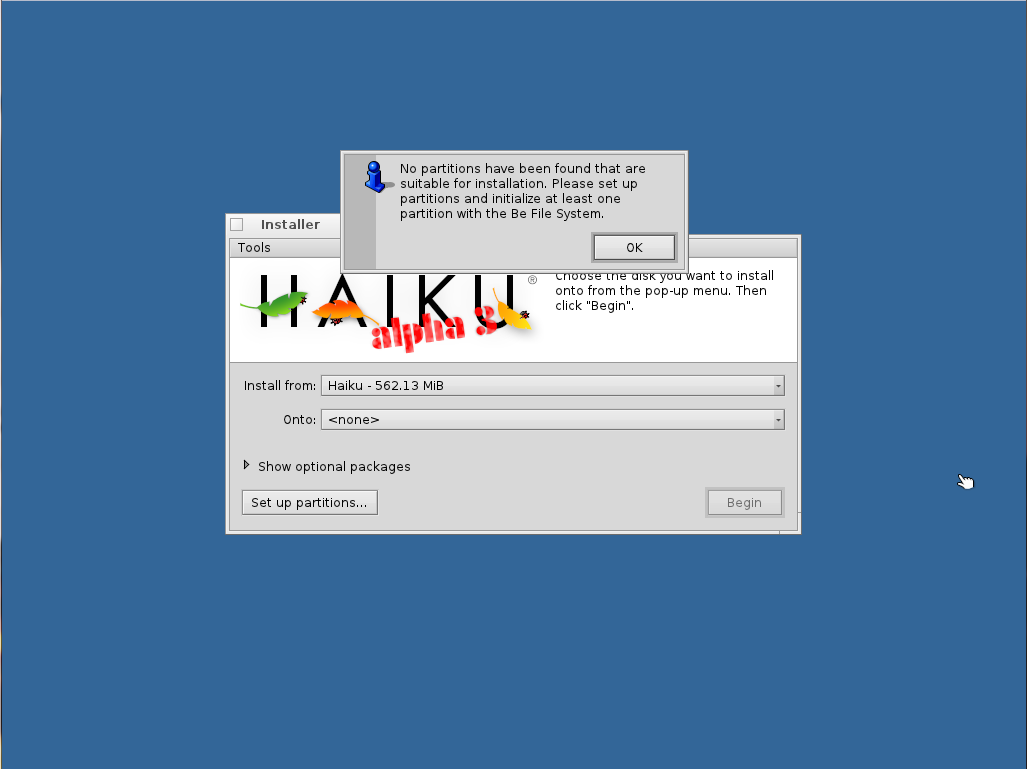
\includegraphics[width=0.9\textwidth]{figs/install-partition.png}
\caption{Partition selection in the Haiku installer.}
\label{fig:install-partition}
\end{figure}

\begin{figure}[h]
\centering
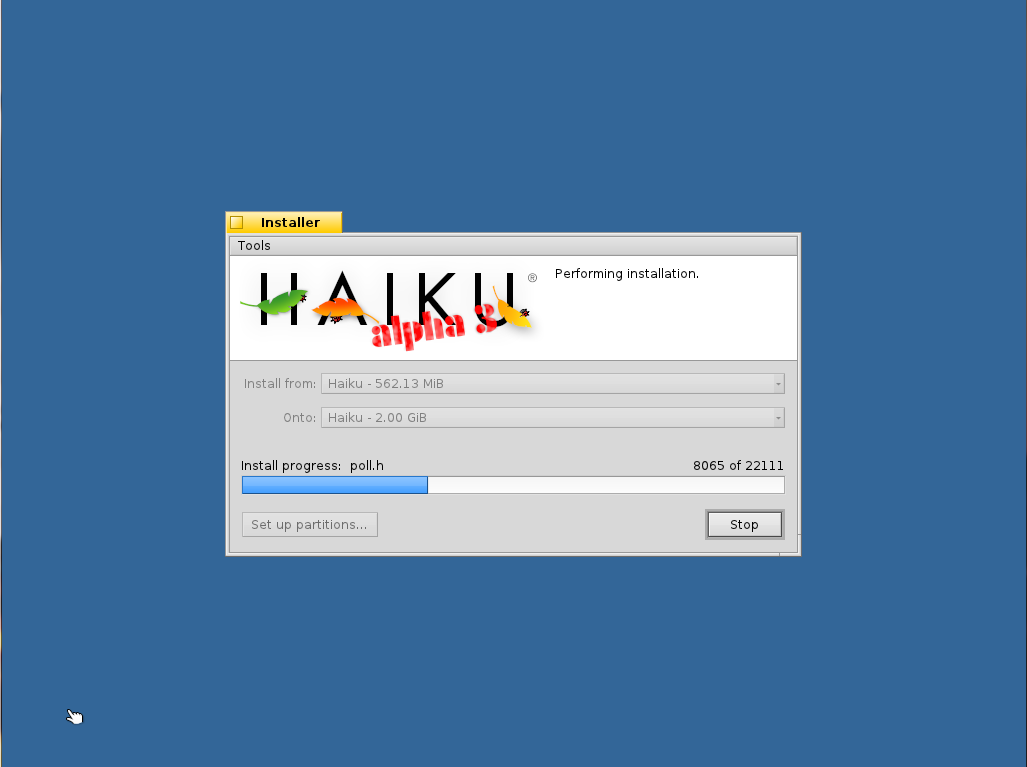
\includegraphics[width=0.5\textwidth]{figs/install-progress.png}
\caption{The Haiku installer copying files and displaying installation
  progress.}
\label{fig:install-progress}
\end{figure}

Installation began by selecting the Haiku disc ISO to be used for the
secondary IDE device in the Storage Settings for my Haiku guest, and a
first boot was initiated.  After a simple language select, a quick and
painless format of my 4GB partition to the Be File system
(\figref{install-partition}), my partition was ready to be selected
from a drop down list and the install could begin
(\figref{install-progress}).  This process could simply not have been
more painless, and there were absolutely no surprises or hurdles to
overcome during the process.  After the progress bar reached the end,
I chose the ``Quit'' option and the system rebooted to be used for the
first time.

\section{Startup}

\begin{figure}[h]
\centering

\includegraphics[width=0.5\textwidth]{figs/startup.png}
\caption{The Haiku boot screen.}
\label{fig:startup}
\end{figure}

The first start-up presents the user with a screen showing the Haiku
logo, and a series of logos that go from monochrome to full color in
sequence to indicate progress during boot-up (\figref{startup}).
Given this execution combined with the artistic styling of the logos,
this is very reminiscent of Maxis' The Sims series of games.

After a noticeably rapid boot process, users familiar with
Haiku's inspiration and spiritual predecessor, BeOS, will be greeted 
instantly with both familiar desktop and icon styling along with the
Tracker, one of very few things that made a direct translation from
BeOS to Haiku as part of being open-sourced in 2001 \cite{HaikuFaq}.

A stark install process gives way to very few options, and with very little
additional effort, Haiku is for all intents and purposes ready for use.  
The time taken from start to finish in setting up an installation of Haiku under
VirtualBox is roughly five minutes.

\section{Basic Operation}

Haiku comes pre-installed with a host of applications that the average
user may use, the most important of which is likely its pre-installed
browser, titled WebPositive.  Haiku is aimed at ``personal
computing,'' and given this vague definition, seems at first glance to fulfill 
the needs of an average light user. The web browser will be the obvious first 
stop for most users looking to get more software and make their Haiku experience 
a more entertaining or productive one.
	
This is where the first very minor problem was encountered, and it was
a network related issue. Haiku refused to recognize the default
network card that VirtualBox had chosen to virtualize, and so a quick
shutdown and modification of this setting to an Intel Pro/1000 MT desktop card 
solved the problem immediately.
	
\begin{figure}[h]
\centering
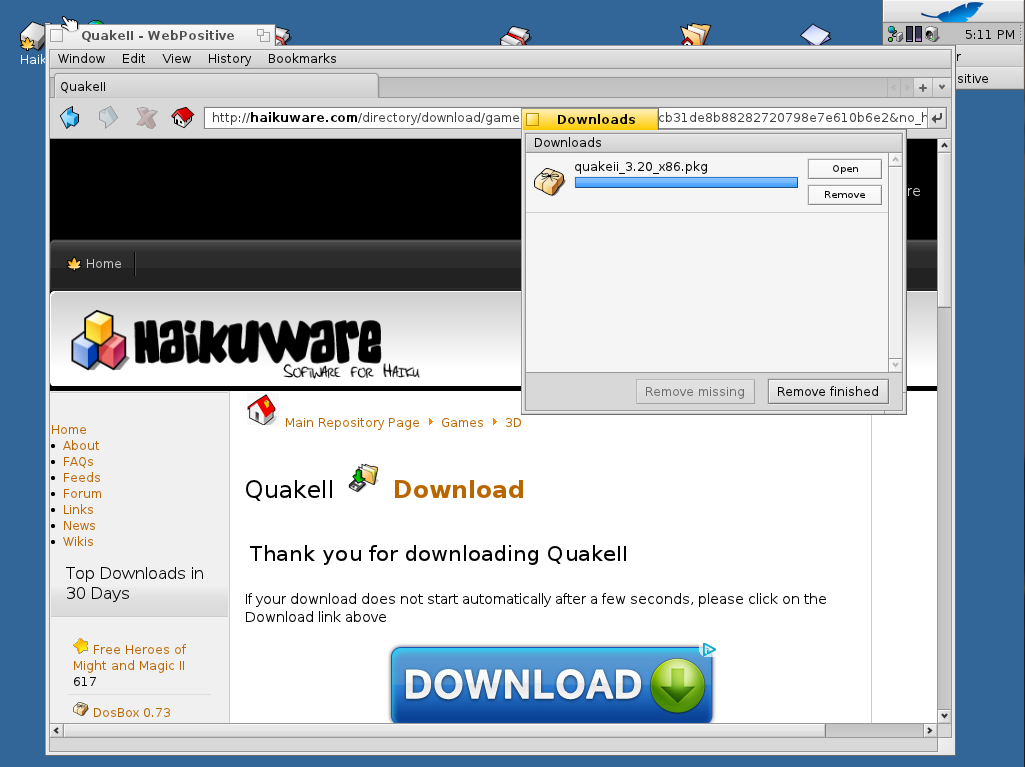
\includegraphics[width=0.9\textwidth]{figs/using-quake-download.png}
\caption{WebPositive, the Haiku web browser, downloading Quake II from
  Haikuware.}
\label{fig:using-quake-download}
\end{figure}

A user looking to expand their selection of installed software will
likely end up at the site Haikuware (located at
http://www.haikuware.com).  Considering my resounding disinterest in
word-processing or productivity programs, I decided to hunt down a
Haiku-compatible version of a classic favourite of mine, id Software's
Quake II(\figref{using-quake-download}).  Interestingly enough, the
claim from the download page at Haikuware for Quake II claims it is
the same version that used to be found on BeDepot.
	
\begin{figure}[h]
\centering
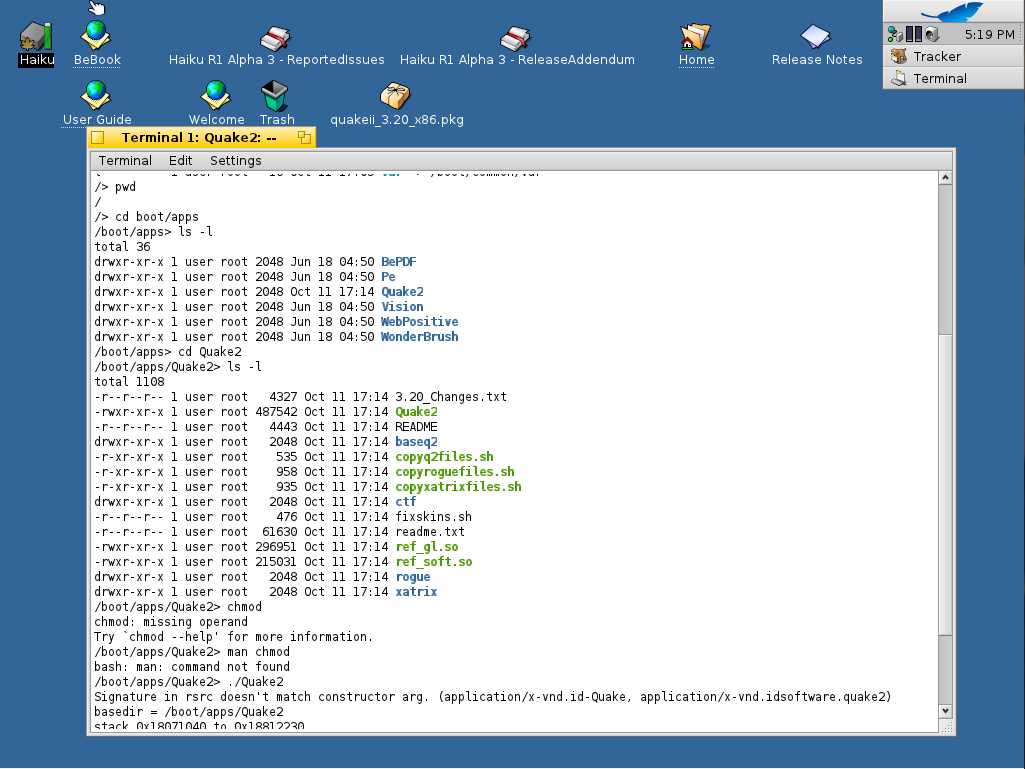
\includegraphics[width=0.9\textwidth]{figs/using-terminal.png}
\caption{A Bash terminal window open in Haiku.}
\label{fig:using-terminal}
\end{figure}

Following the download's completion, the most obvious feature was
its file extension, .PKG. Not recognizing this immediately as a BeOS
installation package, a double click revealed a very simple auto-install
process that I promptly allowed to install to its default directory,
/boot/apps.  The file system in BeOS/Haiku is very similar to that of
a Unix OS, despite Haiku not being a Unix based operating system, and as
such the directory structure looks very similar to Unix systems.
Haiku comes with a Bash terminal, with instantly recognizable Unix commands
such as ls, chmod, pwd, and many others (\figref{using-terminal}).  The
mounting of a CD is automatic, and very easily accessible once
inserted, either from a link on the desktop, or from the root
directory, based on what the name of the CD is.  In this case, I could
access the files on the Quake II CD from /Quake2, and the files from
the installation of BeOS Quake II at /boot/apps/Quake2.

\begin{figure}[h]
\centering
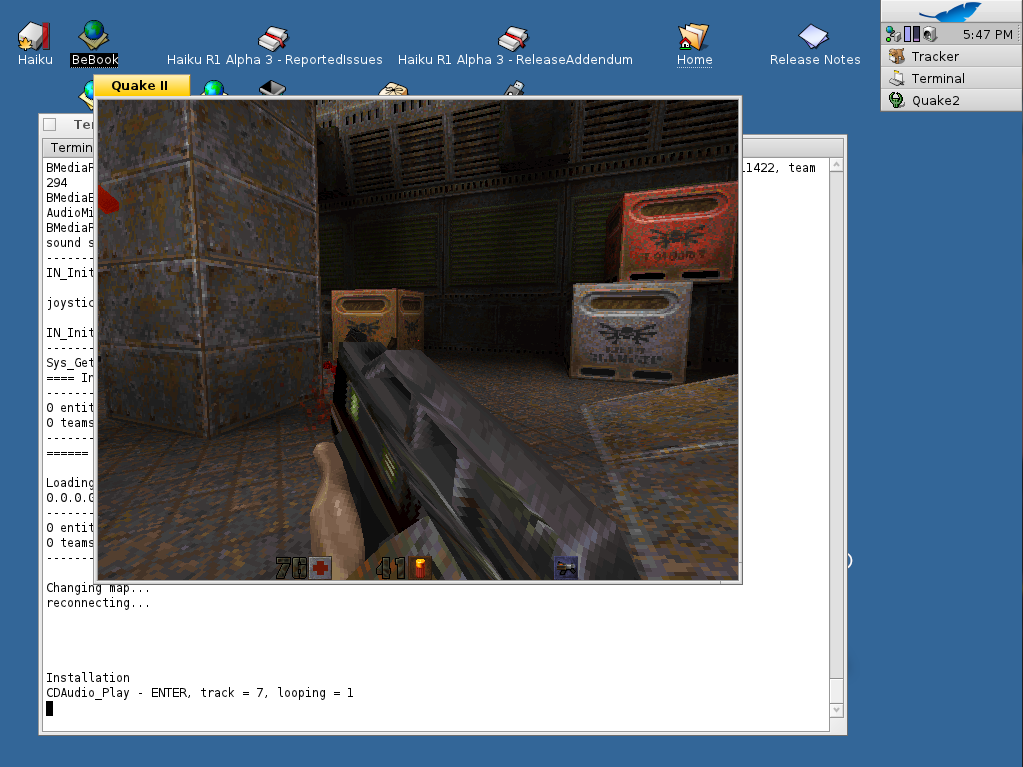
\includegraphics[width=0.5\textwidth]{figs/using-quake-play.png}
\caption{Quake II for BeOS running on Haiku.}
\label{fig:using-quake-play}
\end{figure}
	
After copying the contents of a full Windows installation of Quake II
into Haiku via USB drive (which again was instantly recognized and
mounted), I started it up. Copying from a previously installed Windows
version was necessary because the CD was the Windows version, and availability
of a native BeOS installer is unlikely. 

The first noticeable problems were both
the obviously broken and ear-piercing sound which caused me to mute my
PC, and the excruciatingly slow Mesa software OpenGL implementation
that the game defaulted to.  This is a result of no Guest Additions
and no virtualized OpenGL 3D-acceleration, and as a result, I switched
to pure software rendering mode which ended up working out nicely
(\figref{using-quake-play}).  However, attempting to start a game
causes a crash, and while playing the beginning demo the game will
occasionally crash as well.  I'm not sure if this is a result of it
being a BeOS executable, the fact that I'm running it in VirtualBox,
or just that the BeOS/Haiku executable of Quake II isn't quite ready
for prime time yet.  I was nevertheless still impressed to see it
running in any capacity in Haiku.
	
Most people will at some point want to watch a video on Youtube, or at
least some Flash-based video website.  If Haiku was going to be of any
use to the average personal computer user, I was going to need to
determine whether or not Youtube was a viable option in Haiku.  I set
about trying to download a new browser from Haikuware to spruce up my
browsing experience, and to find out how simple the installation of new
software would be. The unfortunate discovery was that there is a high
degree of difficulty finding and installing new software in Haiku, partly
due to the tiny number of apps available to it that both run natively,
and are easy to install.

There is a small selection of browsers available for Haiku directly
from Haikuware, but they're mostly old versions of browsers
(i.e. Firefox 2.0 since Firefox 3 still isn't fully ported, as well as
older versions of Opera) that still don't have proper plugin support
for things like Flash.  Since Flash is closed-source, open-source
versions of it like Gnash are made, but are still largely unsupported
and not optimal.  This makes something like watching Youtube a more
massive undertaking than most basic users will be capable of, since
getting Flash support in a web browser in Haiku is a task in itself.
This speaks poorly to Haiku's goal to be for ``personal computing,''
considering how many more popular operating systems provide this basic
functionality.

\section{Usage Evaluation}

While a seemingly faithful recreation of the original BeOS and an
impressive piece of work in its own right, Haiku falls short of its
goals to be for ``personal computing'' by simply not having enough
software support and lacking in the excellent package distribution
models that many other more popular operating systems provide.  An
interesting OS, and considering it's open source model could
technically be made to do anything if you felt so inclined, but the
types of users who would delve into source code to coax Haiku into
being more useful aren't the sort of people I feel the Haiku
developers are speaking to when they describe it vaguely as being for
``personal computing.''

\bibliography{haiku}{}
\bibliographystyle{plain}

\end{document}
